%In modern radiotherapy, the precision of dose delivery is essential to maximize the therapeutic effect on cancerous tissues while minimizing exposure to surrounding healthy organs.
%Achieving this balance relies heavily on advanced dose optimization techniques that tailor radiation to each patient's specific anatomical and clinical needs.
\section{Discretization}
The optimization process starts with transforming the continuous nature of both the radiation field and the human body into discrete elements.
This transformation enables computation with modern computers.

\subsection[Bixels]{Fluence Map Discretization: Bixels}

%\begin{figure}
%	\centering
%	\begin{subfigure}[c]{0.95\textwidth}
%		\includegraphics[width=\linewidth]{fluence_discretization_plot.pdf}
%		\caption{2D visualization.}
%		\label{fig:fluence_bixel_2D}
%	\end{subfigure}
%	\\
%	\begin{subfigure}[b]{0.95\textwidth}
%		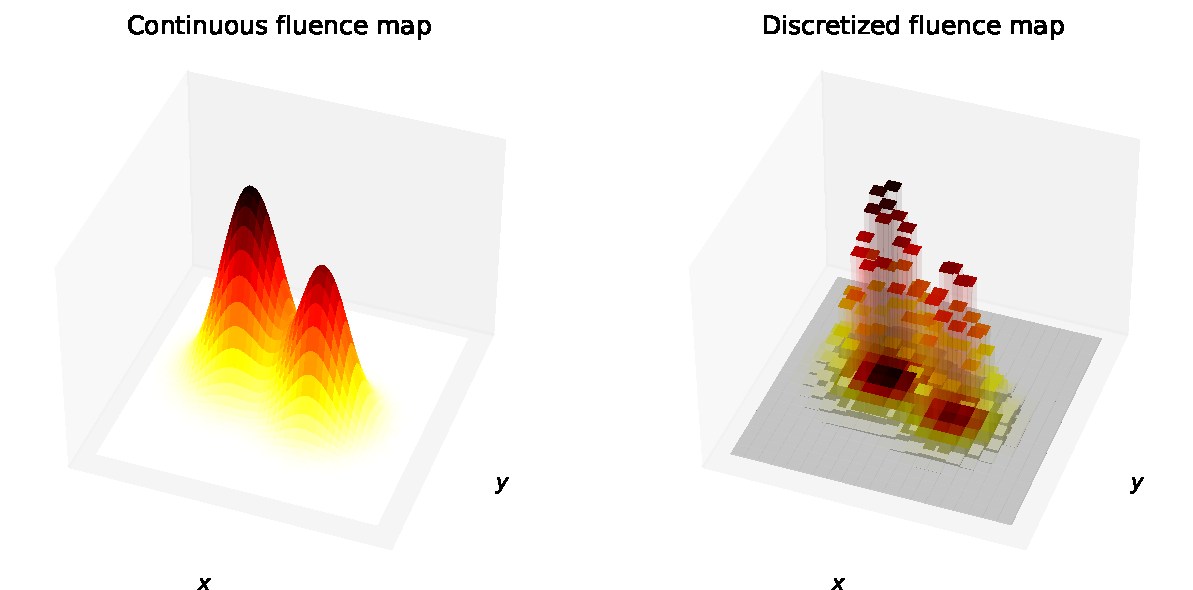
\includegraphics[width=\linewidth]{fluence_discretization_plot3D.pdf}
%		\caption{3D visualization.}
%		\label{fig:fluence_bixel_3D}
%	\end{subfigure}
%	\caption{Example of a fluence discretized to $20 \times 20$ bixels.}
%	\label{fig:fluence_bixel}
%\end{figure}


Fluence maps are broken down into discrete elements called "bixels" (\textbf{be}am \textbf{el}ements).
Bixels represent small and independent beams of radiation.

The width of each bixel is constrained by the width of the multi-leaf collimator leaves.
Modern multi-leaf collimator systems typically have a leaf width of 0.5 cm.

The height of a bixel can be selected arbitrarily, as the leaf can move continuously.
Nevertheless, square bixels (akin to image pixels) are commonly used and will be employed throughout this manuscript.

Bixels whose beams do not affect the planning target volume are typically excluded from calculations to improve computational efficiency.
Activating these bixels could only degrade dose quality by increasing the dose to organs at risk without benefiting the dose distribution within the planning target volume.

\subsection[Voxels]{Human Body Discretization: Voxels}
The human body of the patient is also divided into discrete elements, as it is a three-dimensional object; the elements are "voxels" (\textbf{vo}lume \textbf{el}ements).
Each voxel represents a small portion of tissue within the patient's body, and will determine the granularity of the dose computed.

The maximum resolution of the voxel grid is defined by the planning image, which is typically a CT scan.
It is common practice to resample the planning image to reduce computational demands.
In this manuscript, where new techniques are explored, we have opted to resample the voxel grid to a resolution of 5 mm, ensuring a balance between computational efficiency and accuracy.

Additionally, to further optimize the computational process, only voxels corresponding to the planning target volume (PTV) and organs at risk (OARs) are retained for calculations.
This selective approach reduces unnecessary computation.

\subsection[DI-Matrix]{Dose-Influence Matrix}
The Dose-Influence Matrix (or DI-Matrix) links the discretized fluence map (the bixels values) and the discretized dose distribution within the patient (the dose on each voxel).
This matrix defines how the radiation from each individual bixel influences the dose delivered to every voxel in the patient's body.

We start by converting the 2D fluence map, composed of individual bixel values, into a column vector $b$.
Similarly, we represent dose distribution in the patient's 3D space as a vector $\mathbf{d}$, where each entry corresponds to the dose in a specific voxel.
The DI-Matrix $L$ governs the relationship between these vectors $\mathbf{b}$ and $\mathbf{d}$ via the matrix-vector multiplication $\mathbf{d} = L\mathbf{b}$.
This mathematical operation computes the total dose at each voxel by summing the contributions from all active bixels (here, we assume that the effect of bixels is linear).

The DI-Matrix is constructed by simulating the radiation delivered by each individual bixel.
For each bixel, the jaws of the multi-leaf collimator are virtually opened to allow only that specific beamlet to go through.
A radiation transport model calculates the dose deposited in each voxel, considering the beam's spread and attenuation as it travels through the body.
The resulting 3D dose deposition fills one column of the matrix $L$, corresponding to that bixel's influence on all voxels.
Repeating this process for each bixel generates the entire DI-Matrix.

The accuracy of the dose calculation depends on the precision of the DI-Matrix.
Simple models like pencil beam approximations, which assume a linear trajectory with minimal scattering, are considered too coarse.
In contrast, more advanced simulations, such as Monte Carlo methods, provide a detailed and accurate dose calculation, although at a higher computational cost.
In this manuscript, we employ collapsed cone convolution techniques, which balance efficiency and accuracy.

\section{Naive Optimization Method}
A natural starting point in dose optimization is to attempt to directly achieve the delivery of a uniform dose, equal to the prescription, on all voxels within the PTV, and no dose elsewhere.
We can attempt to find the bixels values delivering this dose by solving a least squares problem.
We attempt to find the fluence map $\mathbf{b}$ that minimizes the difference between the actual dose $\mathbf{d}$ and the target dose $\mathbf{d}_{\text{target}}$, which is set to the prescribed dose within the PTV.

Formally, the optimization problem can be stated as:
$$ \min_\mathbf{b} \| \mathbf{d}_{\text{target}} - L\mathbf{b} \|^2 $$

where $\mathbf{d}_{\text{target}}$ is the target dose vector, defined as follow for a prescription of $p$Gy:
$$ \mathbf{d}_{\text{target}} = p \cdot  \mathds{1}_{\text{PTV}} $$

Here, $\mathds{1}_{\text{PTV}}$ is the indicator vector for PTV that is equal to $1$ for voxels within the PTV and $0$ elsewhere.

To solve this problem, we perform a least squares minimization to find the optimal fluence map $\mathbf{b}$, where the matrix-vector multiplication $L\mathbf{b}$ yields the dose distribution $\mathbf{d}$ across the entire patient volume.

However, this method is often inadequate in practice, as it attempts to solve the system based solely on the prescribed dose within the PTV, while neglecting any constraints on doses to the organs at risk (OARs).
Since no constraints are imposed on the OAR doses, this naive optimization can result in high doses to critical structures, leading to unacceptable treatment plans.
As a result, more sophisticated optimization methods that incorporate dose constraints on OARs and account for dose-volume constraints are necessary to achieve clinically viable treatment plans.
% add 3D dose & DVHs of dose obtained using this technique

\section{Constraints and Importance Factors}
In order to obtain clinically acceptable doses, we need to incorporate the clinical aims in the optimization.

\subsection{Constraints Formulation}
Different organs exhibit varying sensitivities to radiation, which influence their dose tolerance limits \cite{Withers1988} \cite{ICRU83}.
Normal tissues are categorized as serial, parallel, or mixed, based on the functional organization of their sub-units.
This classification determines the appropriate absorbed dose limits for normal tissues.

Serial organs (figure \ref{fig:serial_organ}), such as the spinal cord or esophagus, are characterized by a functional dependence on the integrity of every sub-unit.
Damage to even a tiny region in these tissues can result in the loss of the organ's overall function.
In contrast, parallel organs (figure \ref{fig:parallel_organ}), such as the lung or liver, possess a reserve capacity where damage to a portion of the tissue does not necessarily impair overall function, as long as a critical volume remains intact.

\begin{figure}
	\begin{subfigure}{0.6\textwidth}
		\centering
		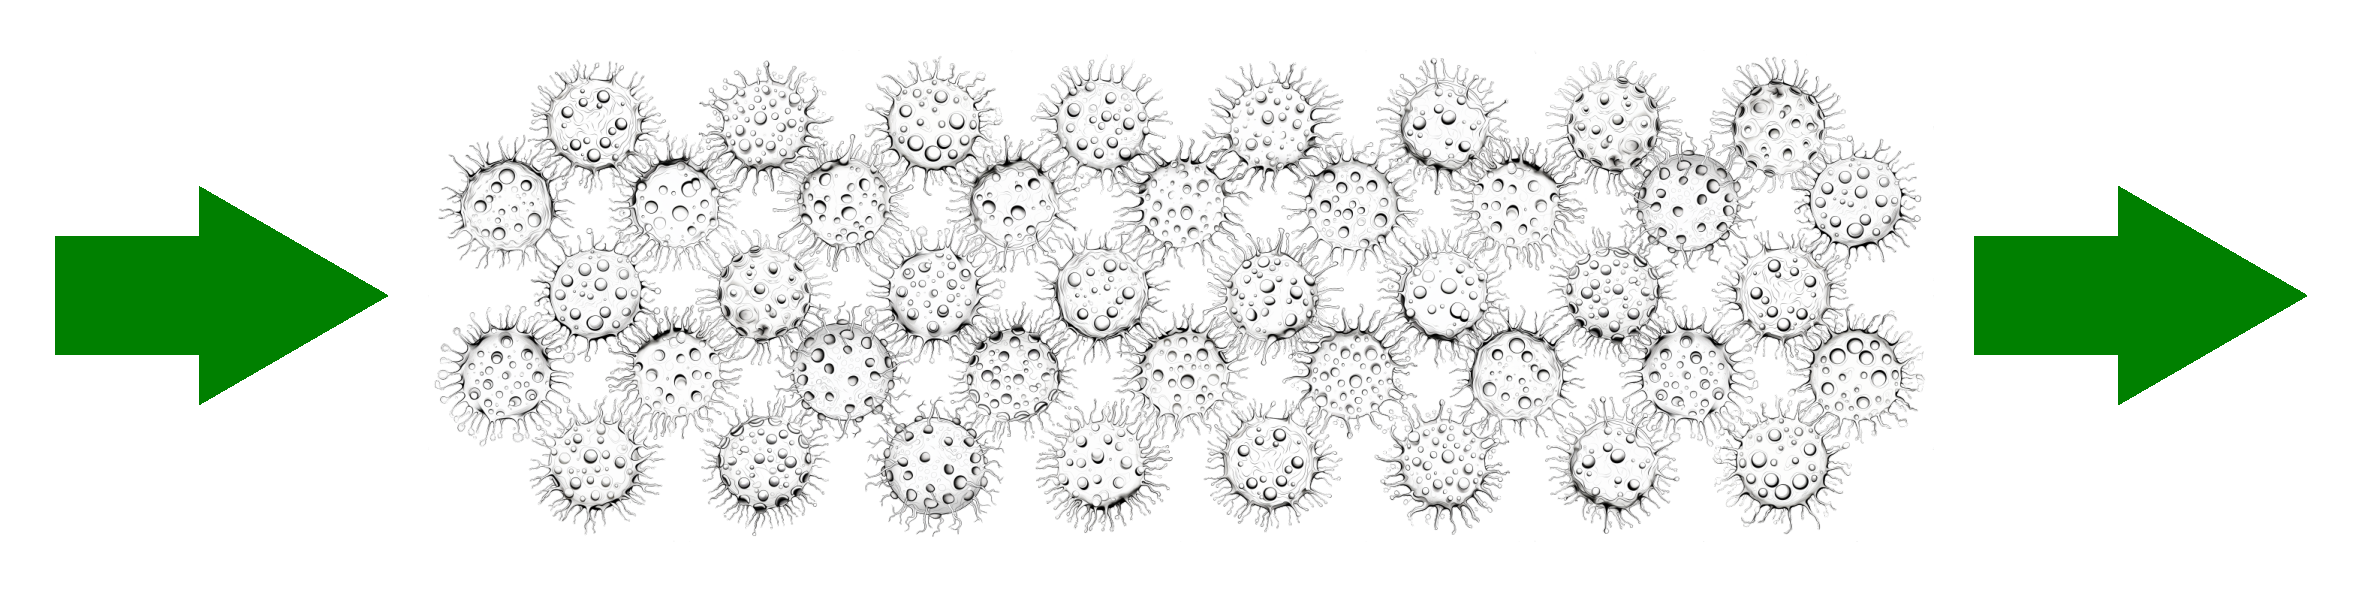
\includegraphics[width=0.9\textwidth]{serial_organ.pdf}
		\vspace{4mm}
		\caption{Organ functioning in a serial-like way.}
		\label{fig:serial_organ}
	\end{subfigure}
	\hfill
	\unskip\ \vrule\
	\hfill
	\begin{subfigure}{0.38\textwidth}
		\centering
		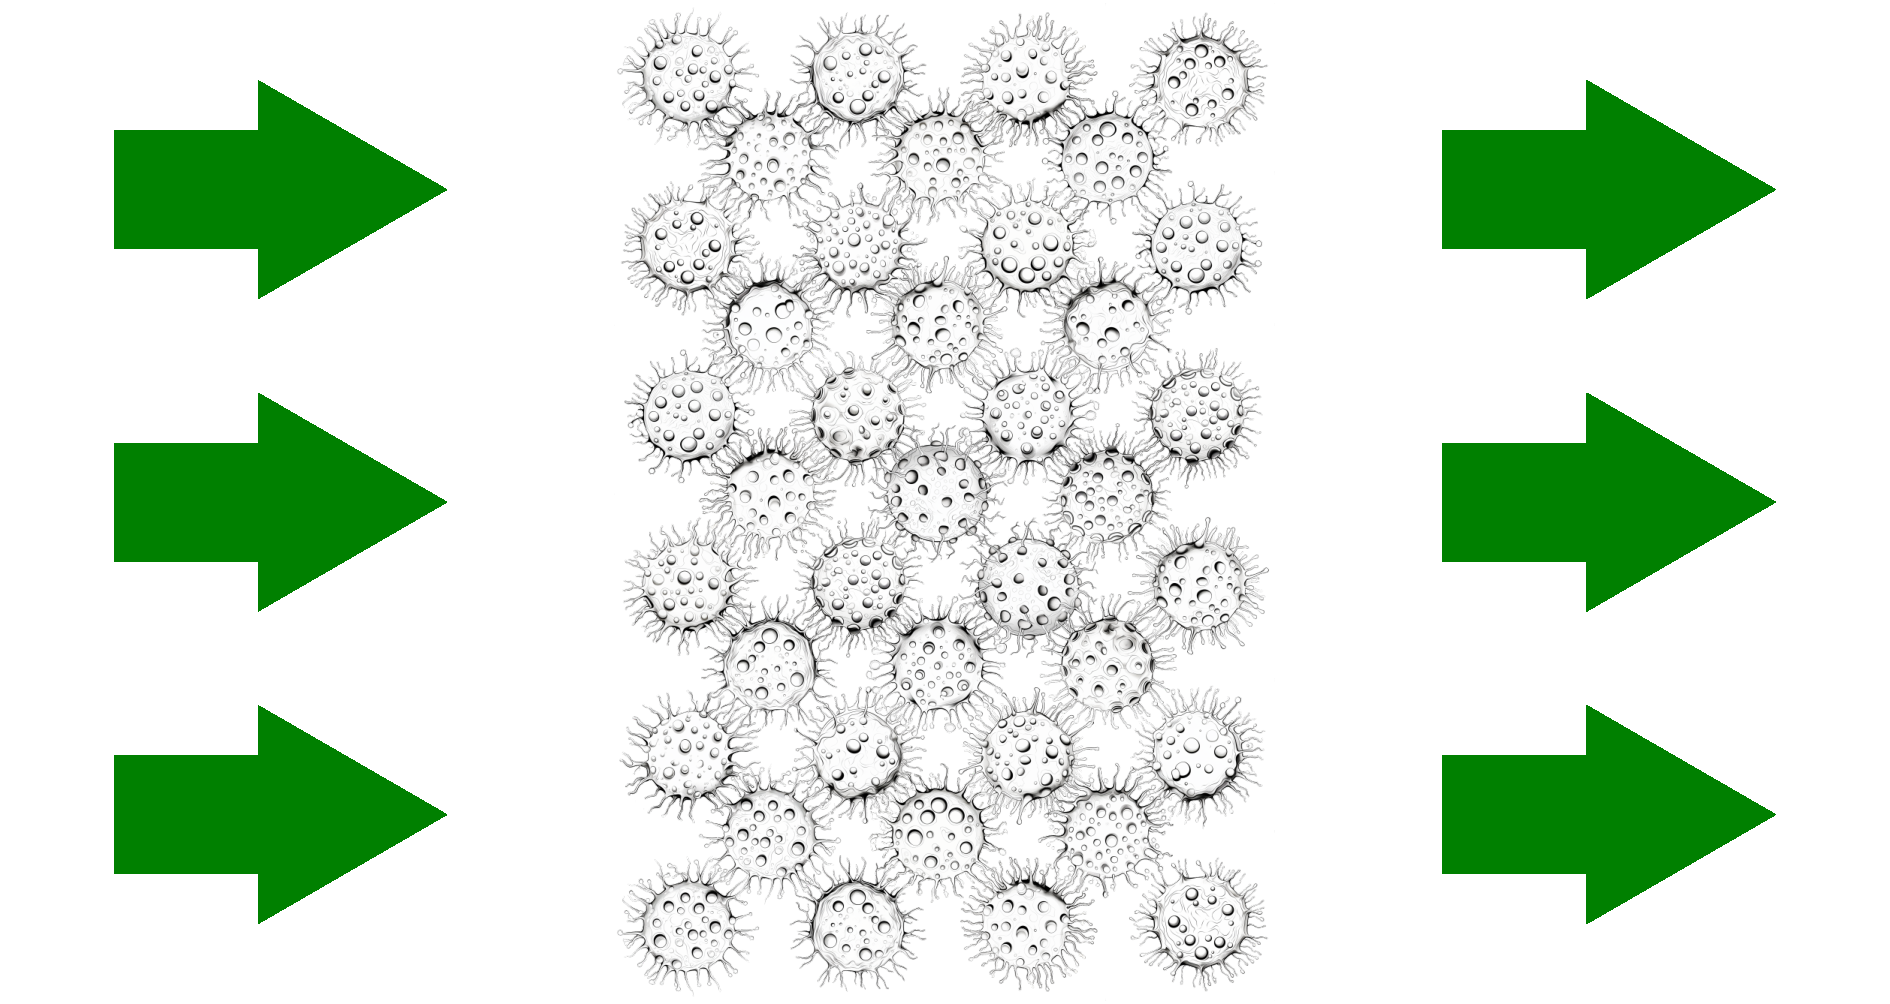
\includegraphics[width=0.9\textwidth]{parallel_organ.pdf}
		\caption{Organ functioning in a parallel-like way.}
		\label{fig:parallel_organ}
	\end{subfigure}
	\caption{Organs functioning types.}
	\label{fig:serial_parallel_organ}	
\end{figure}

We define two DVH value measures $V_X$ and $D_{X\%}$ for a structure $S$.
For a given dose $d: \R^3 \to \R^+$, $V_X$ is defined as the volume of the three dimensional structure $S \subseteq \R^3$ that receives a dose equal to or higher than $X$, that is:
$$ V_X = \frac{\vol{\left\lbrace p \in S \subset \R^3 \mid d(p) \geq X \right\rbrace}}{\vol{S}}.$$
This can be approximated using the discretized dose $\mathbf{d}$:
$$ V_X \approx \frac{ \#{\left\lbrace v \in S \mid \mathbf{d}_v \geq X \right\rbrace}}{\#\left\{ v \in S \right\}}$$
with $v \in S$ voxels of the structure $S$, $\mathbf{d}_v$ the dose of $\mathbf{d}$ associated with voxel $v$, and $\#$ refers to voxel count.

Similarly, we define $D_{X\%}$ as the minimal dose (in Gy) delivered to that the $X\%$ most irradiated region of the structure, that is:
$$D_{X\%} = \min \left\lbrace d(p) \mid p \in S_{X\%} \right\rbrace$$
where $S_{X\%} \subseteq S$ is the $X\%$ most irradiated region of $S$.
$$D_{X\%} \approx \min \left\lbrace \mathbf{d}_v \mid v \in S_{X\%} \right\rbrace$$
where $v \in S_{X\%}$ are the $X\%$ most irradiated voxels of $S$.

This $D_{X\%}$ can also be defined as the maximal dose $D$ such that $V_D$ the volume of $S$ that receives a dose equal to or higher than $D$ is greater than or equal to $X$:
$$D_{X\%} = \max \left\lbrace D \in \R^+ \mid V_D \geq X\% \right\rbrace.$$
The DVH curve is the plot of $x \mapsto V_x$ on the range of $d$.

For parallel-like structures, dose–volume reporting specifying $V_D$ is commonly used, with $D$ adapted to the specific organ.
For instance, \cite{Graham1995} demonstrated a correlation between the incidence and severity of lung pneumonitis and $V_{20 \text{ Gy}}$, the volume of the lung receiving more than 20 Gy.
Additionally, in parallel-like structures, the median absorbed dose ($D_{50\%}$), provides a valuable measure of the total dose delivered to the organ at risk.

For serial-like organs, it is recommended to report $D_{2\%}$ as the maximum absorbed dose, as $D_{0\%}$ is subject to noise.

Finally, for organs with a mixed parallel-serial structure, it is advised to report $D_{50\%}$, $D_{2\%}$, and $V_D$, with $D$ selected based on the threshold beyond which there is a significant risk of serious complications.

\begin{figure}
	\begin{subfigure}[b]{0.48\textwidth}
		\caption{Irradiation of organs at risk with one heat point.}
		\label{fig:organ_radiation_point}
		\centering
		\vspace{3mm}
		\hspace{1.2cm}
		Treatment Dose
		\\
		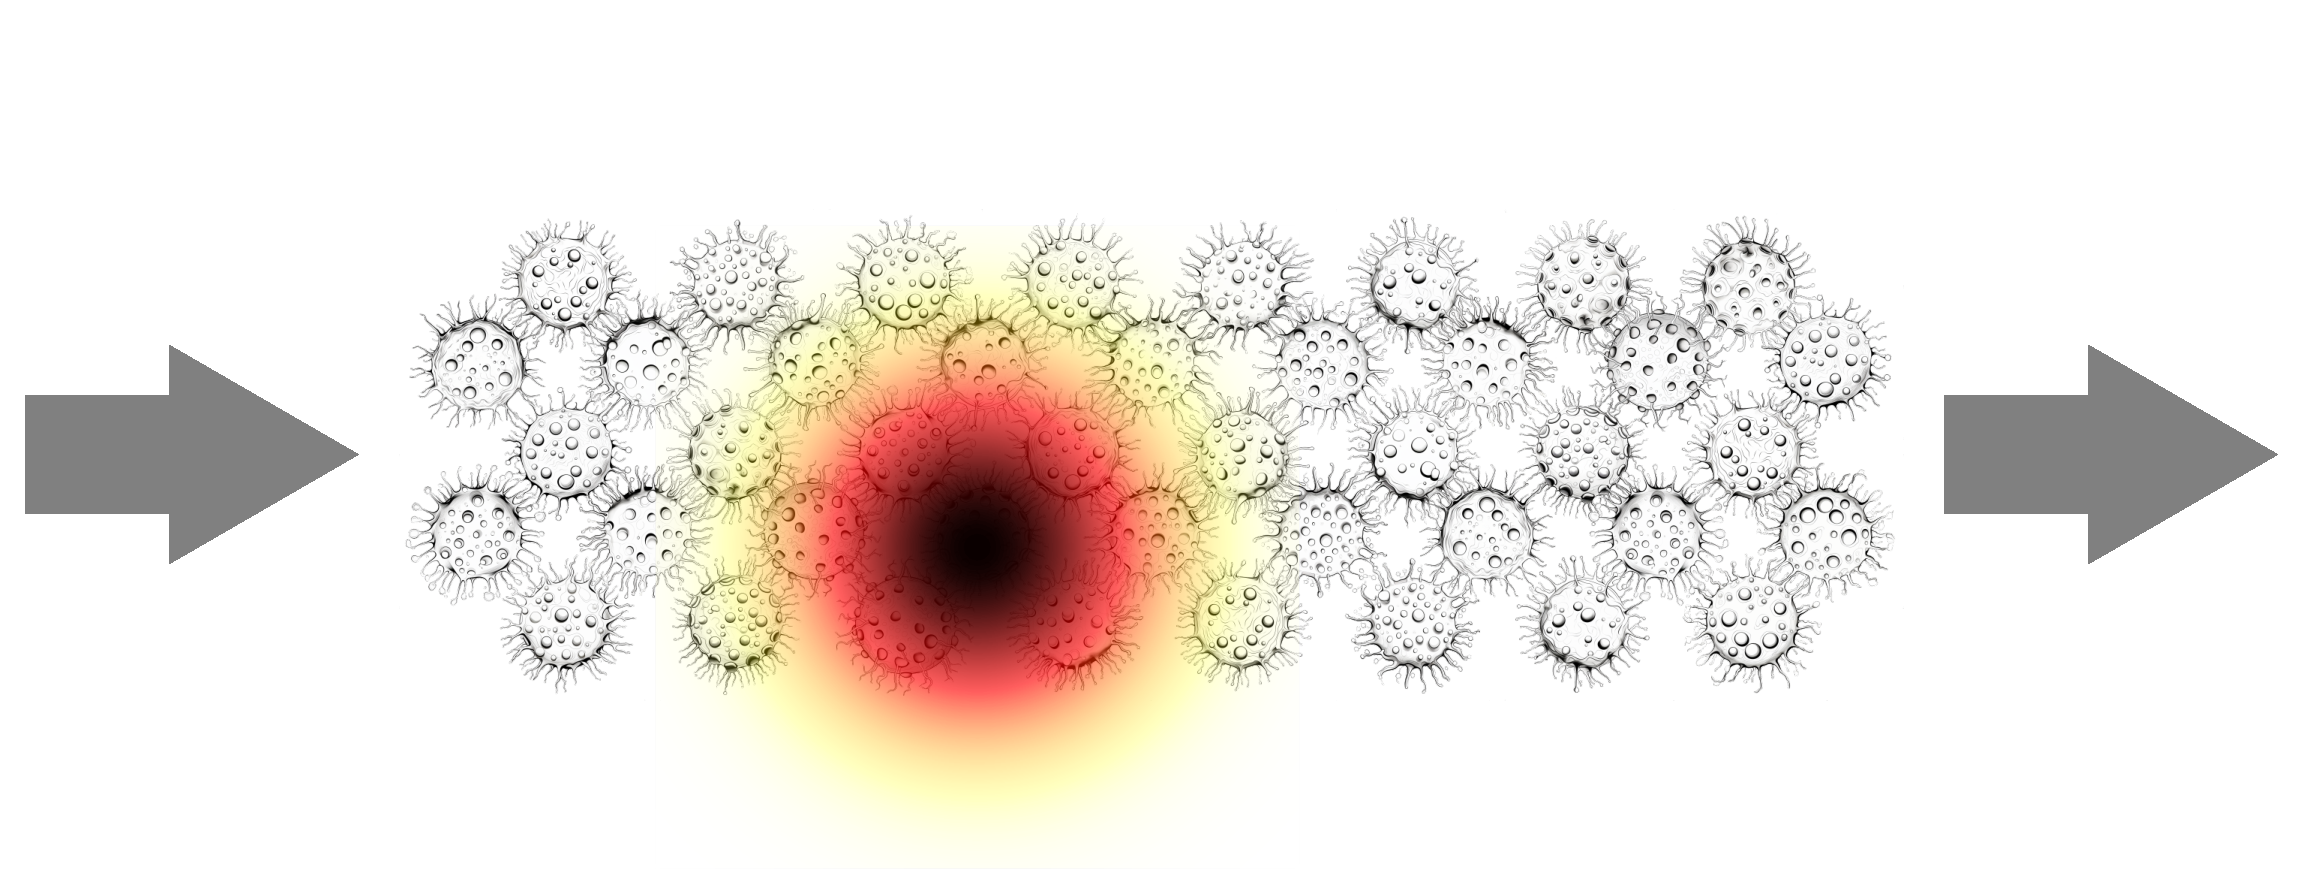
\includegraphics[width=0.55\textwidth]{serial_heat_point.pdf}
		\vbar
		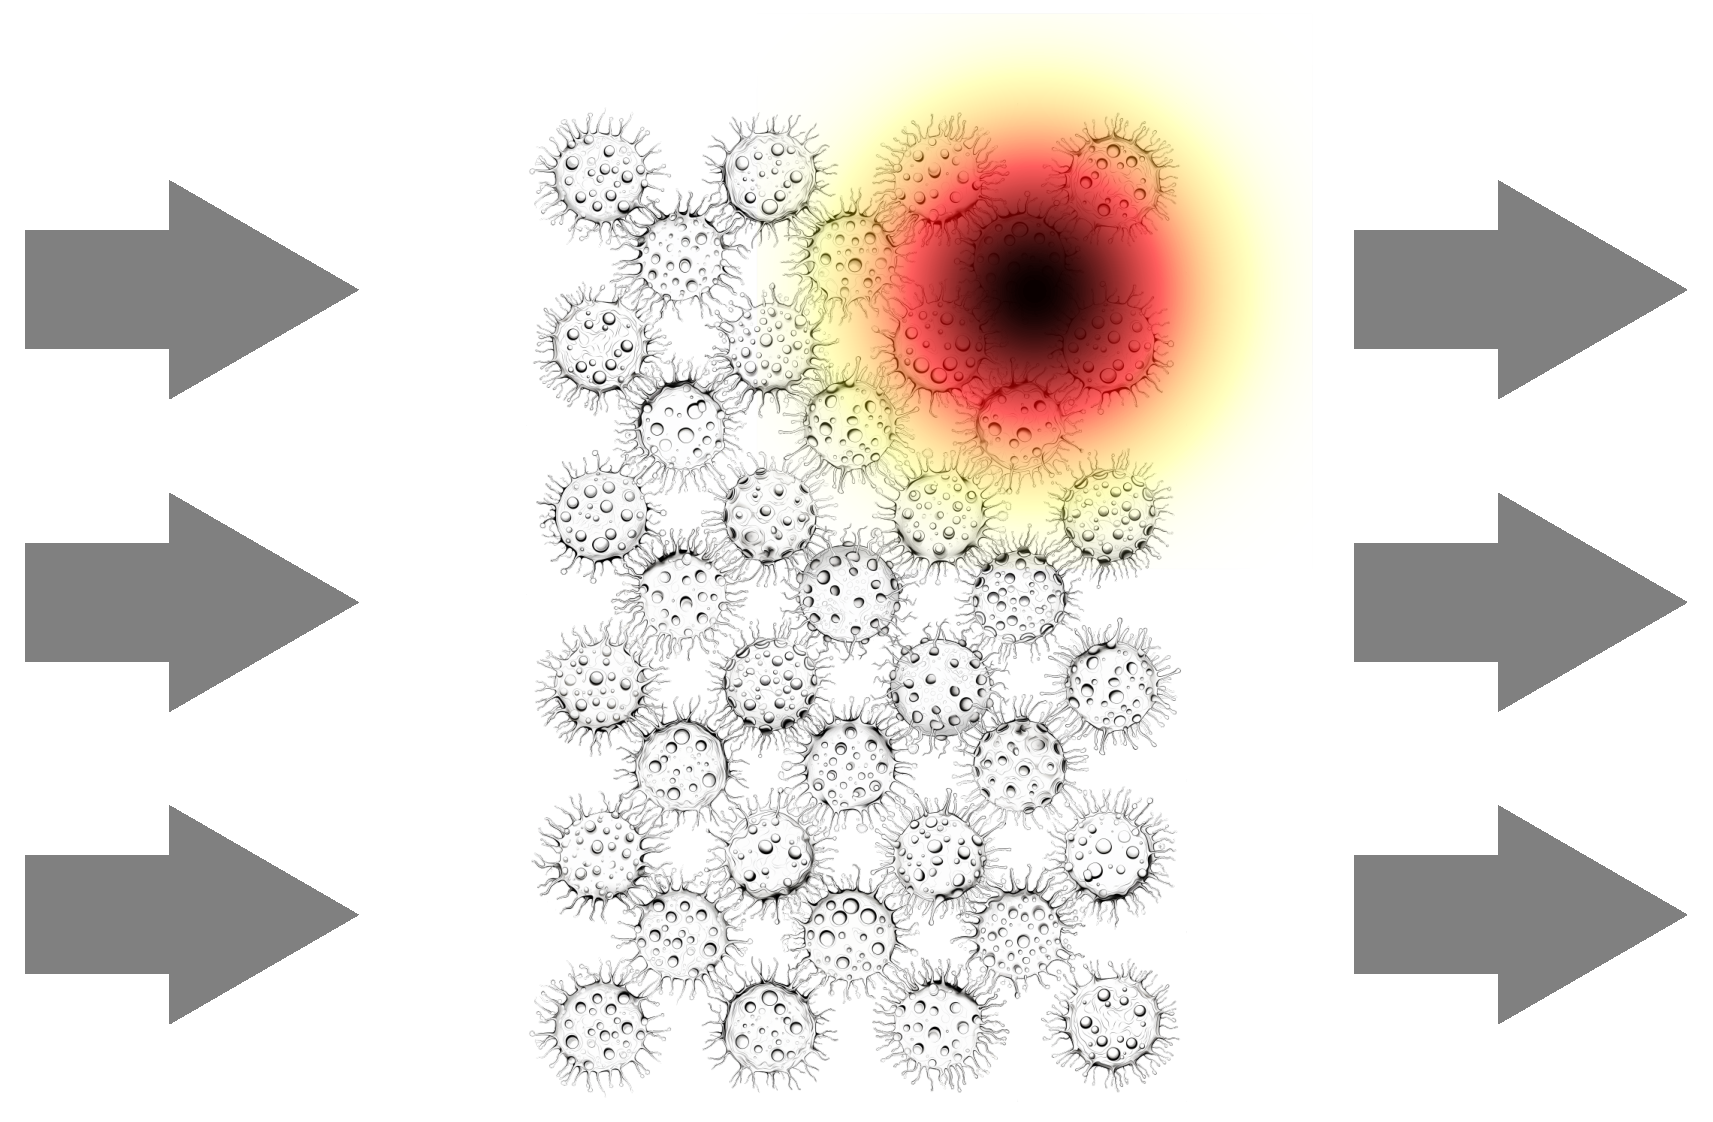
\includegraphics[width=0.35\textwidth]{parallel_heat_point.pdf}
		\\
		\hspace{1.1cm}
		Post Treatment
		\\
		\noindent
		\begin{subfigure}[b]{0.55\textwidth}
			\addtocounter{subfigure}{-1}
			\renewcommand\thesubfigure{\alph{subfigure}1}
			\centering
			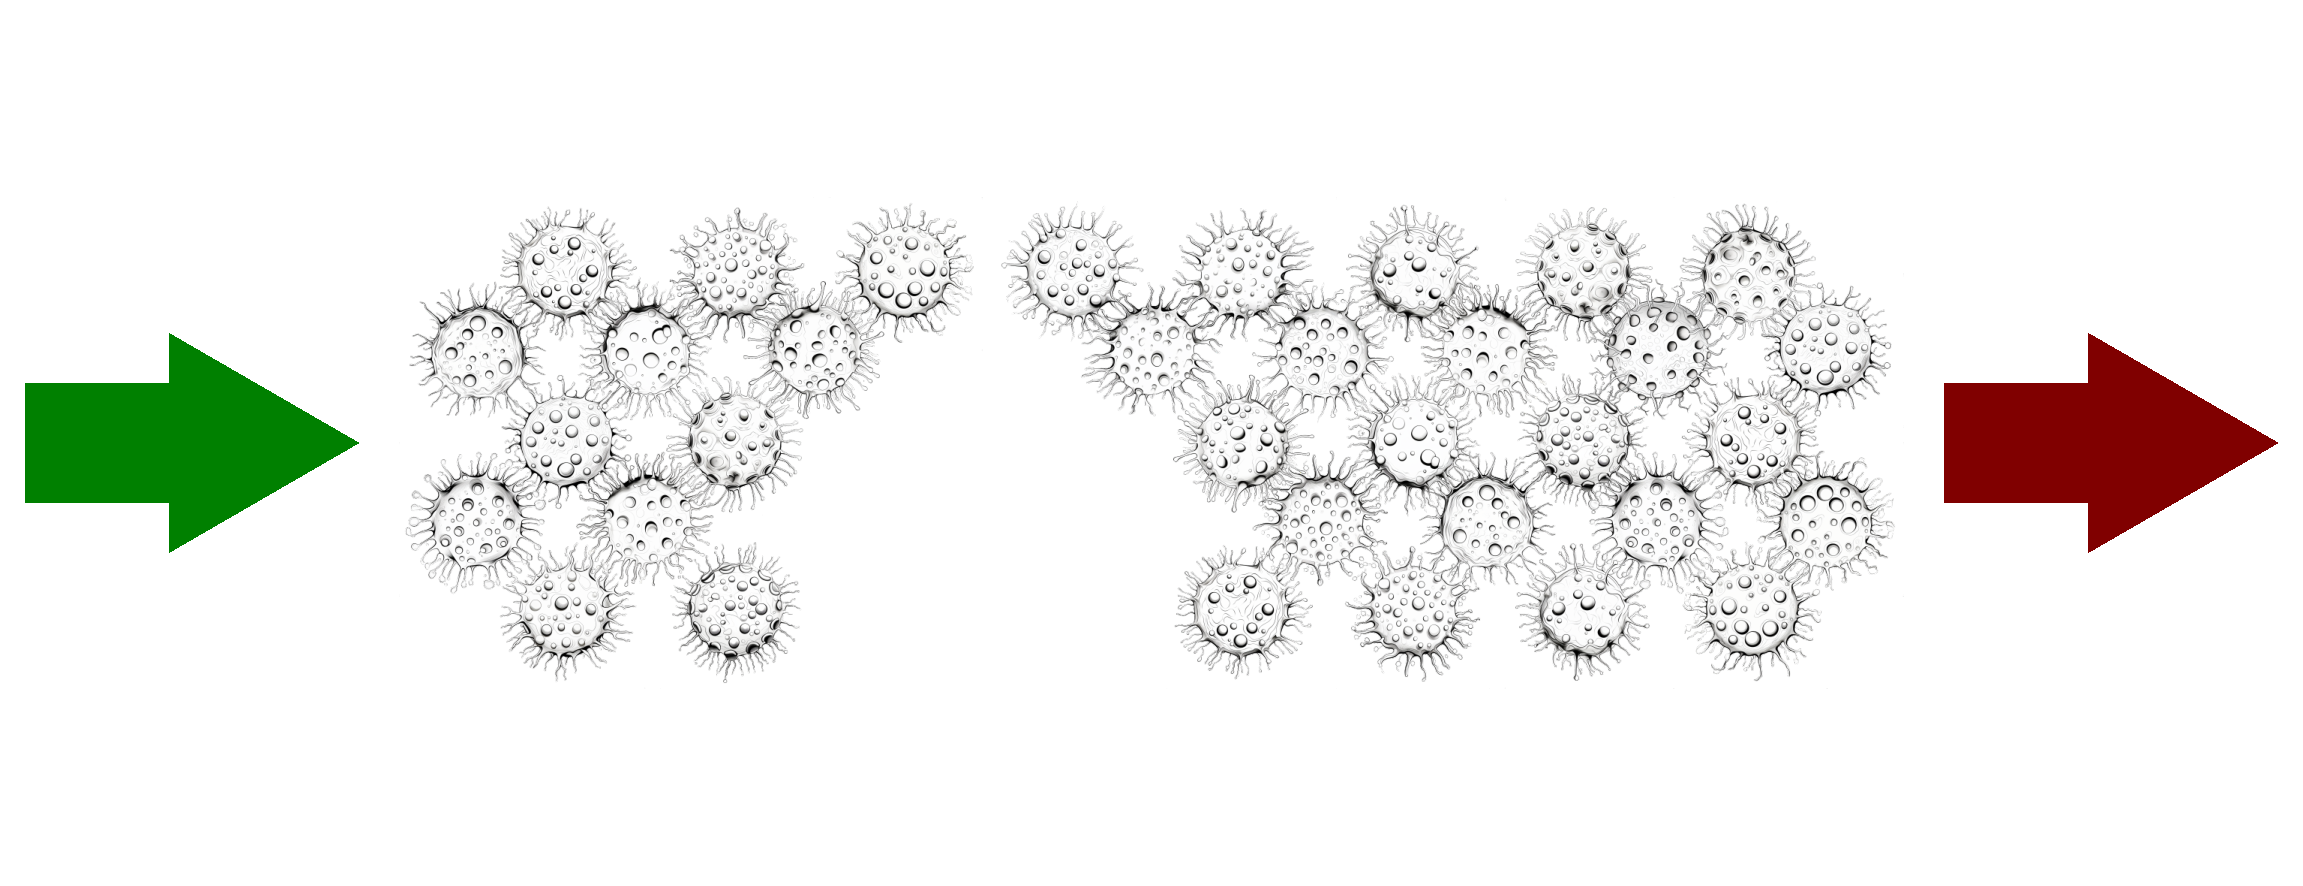
\includegraphics[width=\textwidth]{serial_heat_point_post.pdf}
			\vspace{0.5mm}
			\caption{Serial organ dies.}
		\end{subfigure}
		\vbar
		\begin{subfigure}[b]{0.35\textwidth}
			\addtocounter{subfigure}{-1}
			\renewcommand\thesubfigure{\alph{subfigure}2}
			\centering
			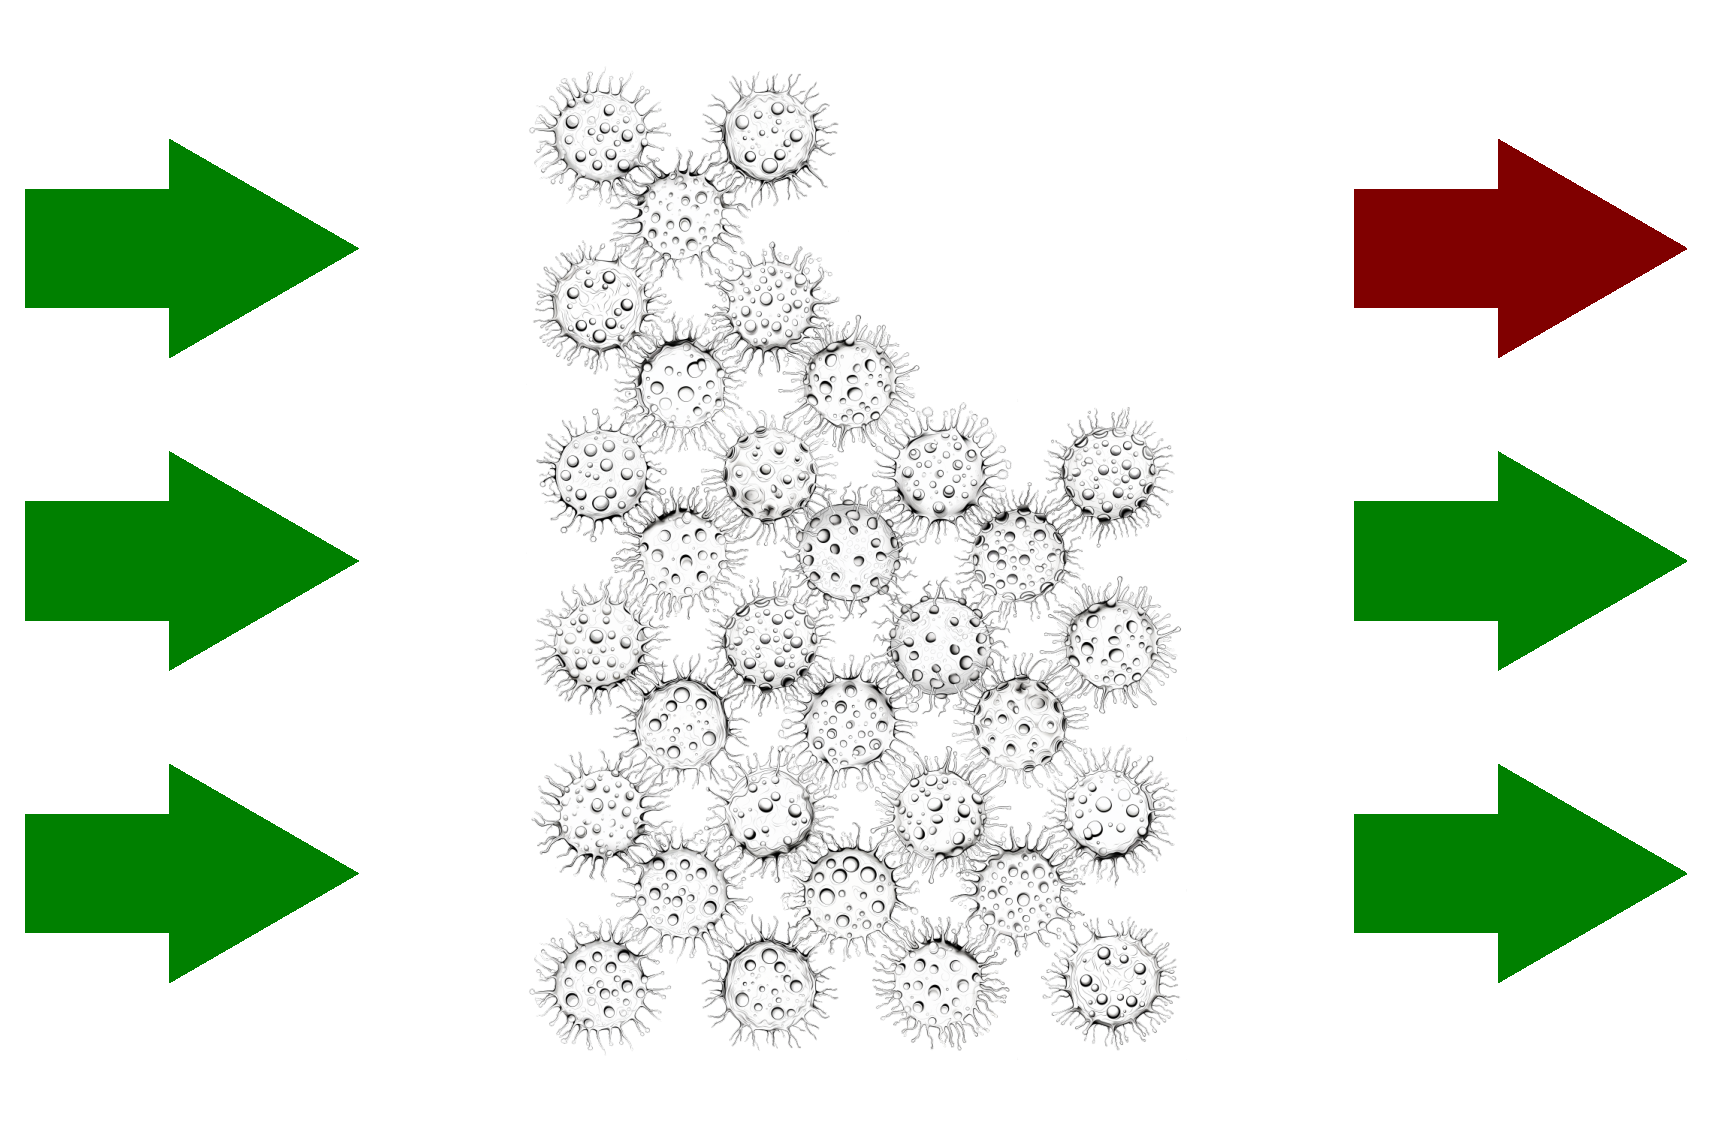
\includegraphics[width=\textwidth]{parallel_heat_point_post.pdf}
			\caption{Parallel organ survives.}
		\end{subfigure}	
	\end{subfigure}
	\vbar
	\begin{subfigure}[b]{0.48\textwidth}
		\caption{Irradiation of organs at risk with spread heat dose.}
		\label{fig:organ_radiation_square}
		\centering
		\vspace{3mm}
		\hspace{1.2cm}
		Treatment Dose
		\\
		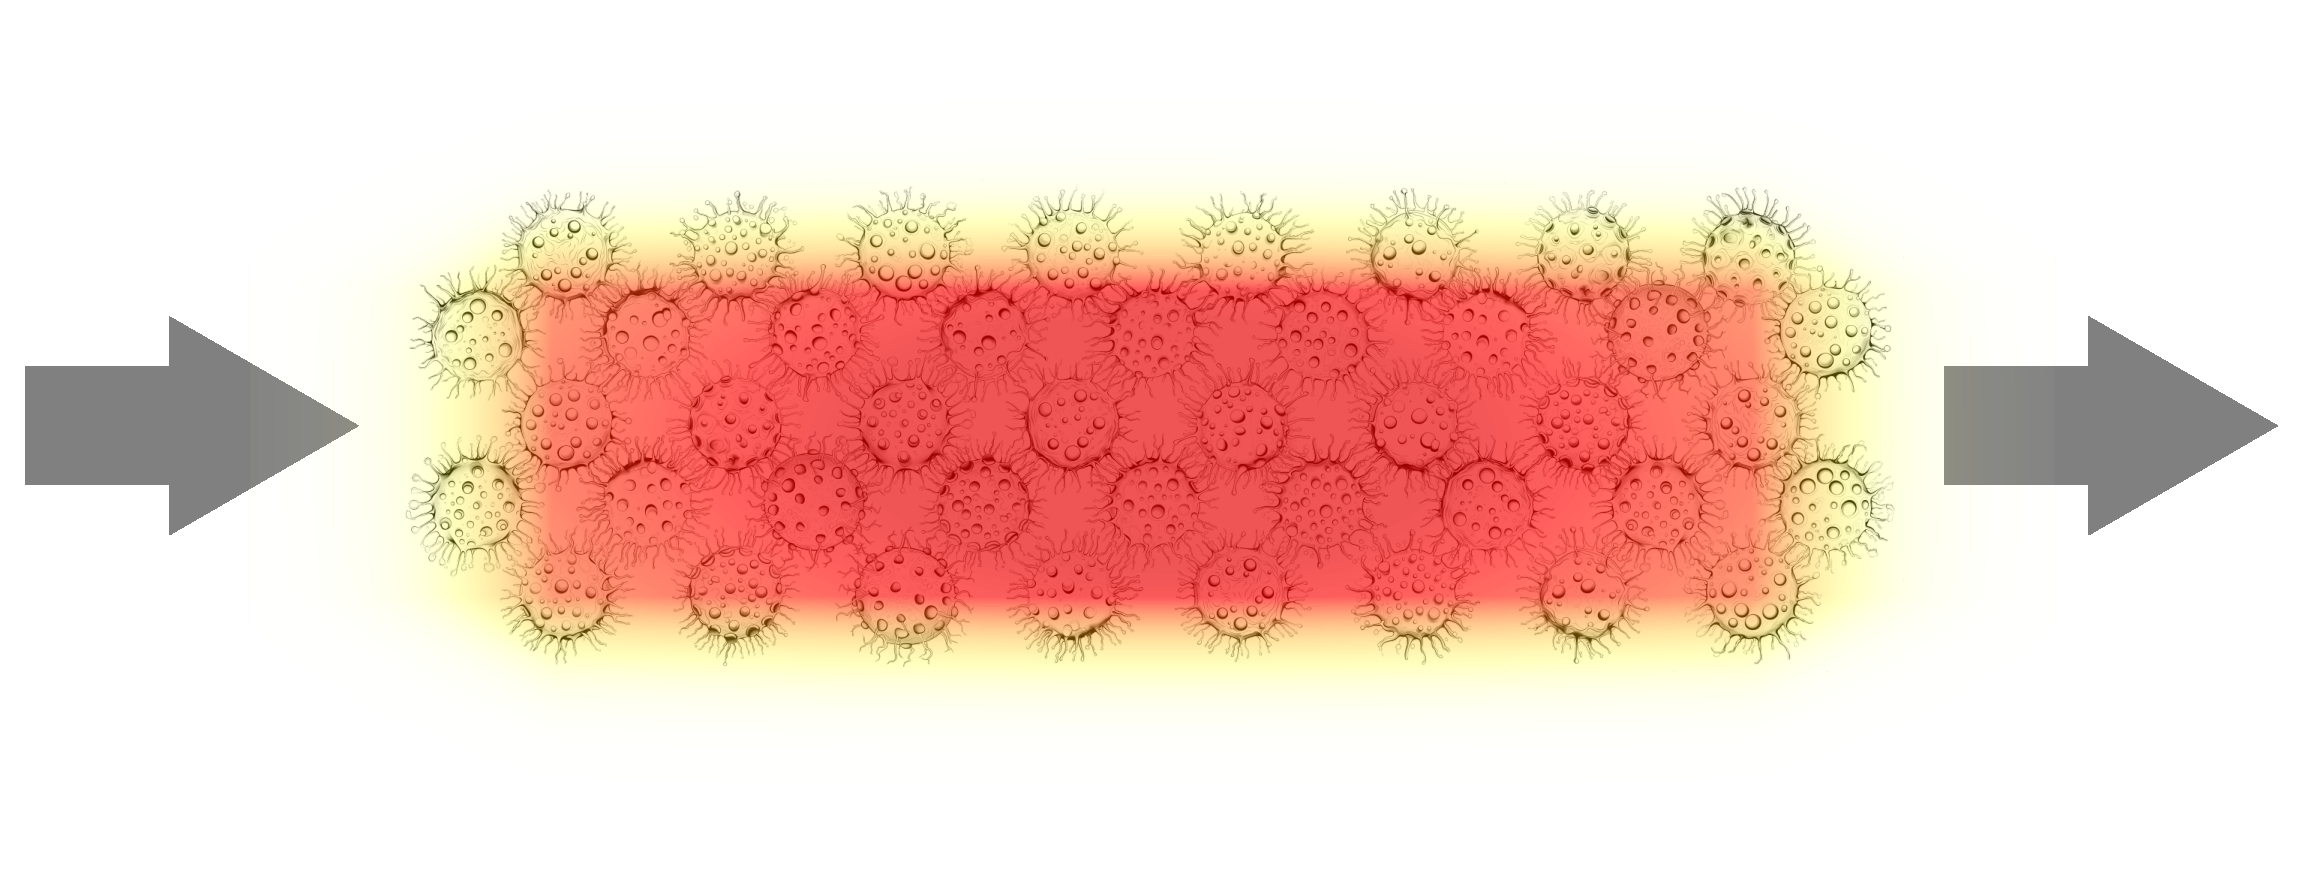
\includegraphics[width=0.55\textwidth]{serial_heat_square.pdf}
		\vbar
		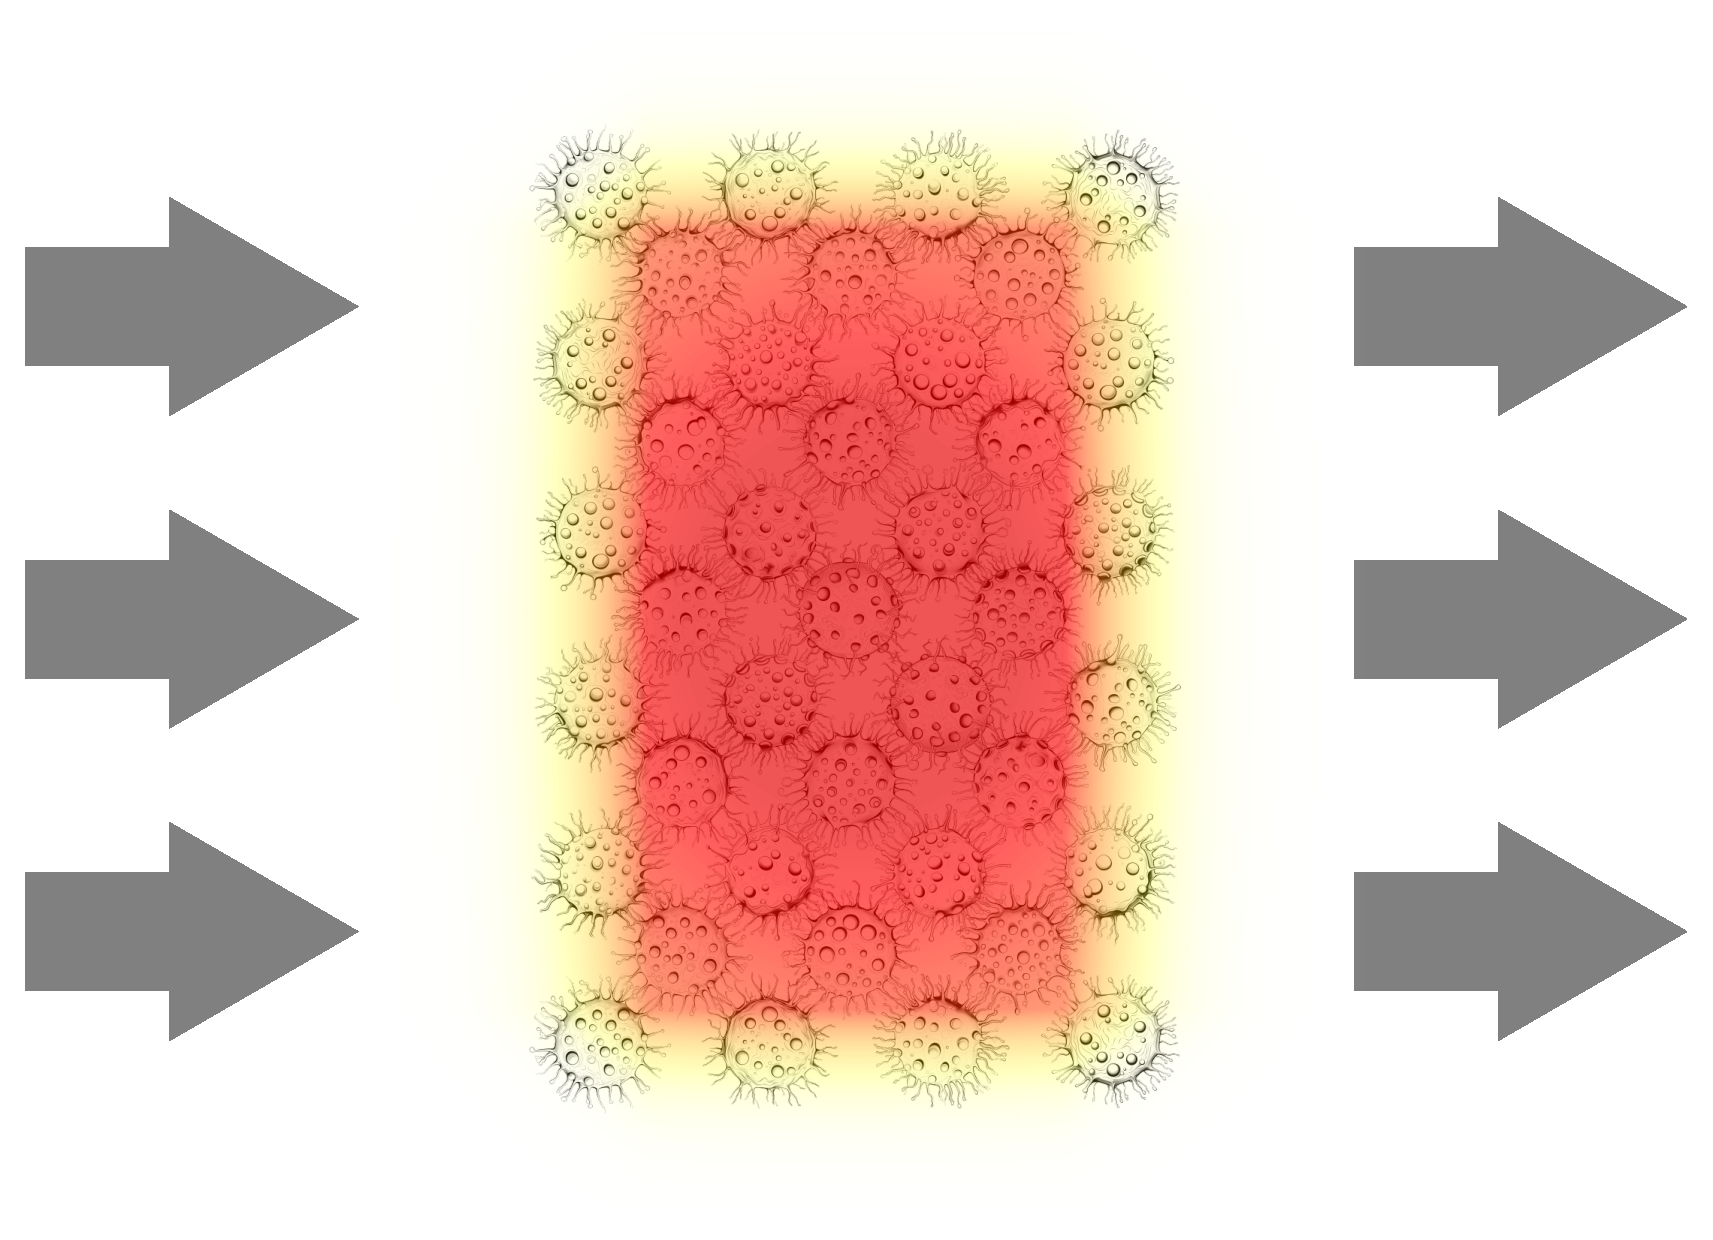
\includegraphics[width=0.35\textwidth]{parallel_heat_square.pdf}
		\\
		\hspace{1.1cm}
		Post Treatment
		\\
		\noindent
		\begin{subfigure}[b]{0.55\textwidth}
			\addtocounter{subfigure}{-1}
			\renewcommand\thesubfigure{\alph{subfigure}1}
			\centering
			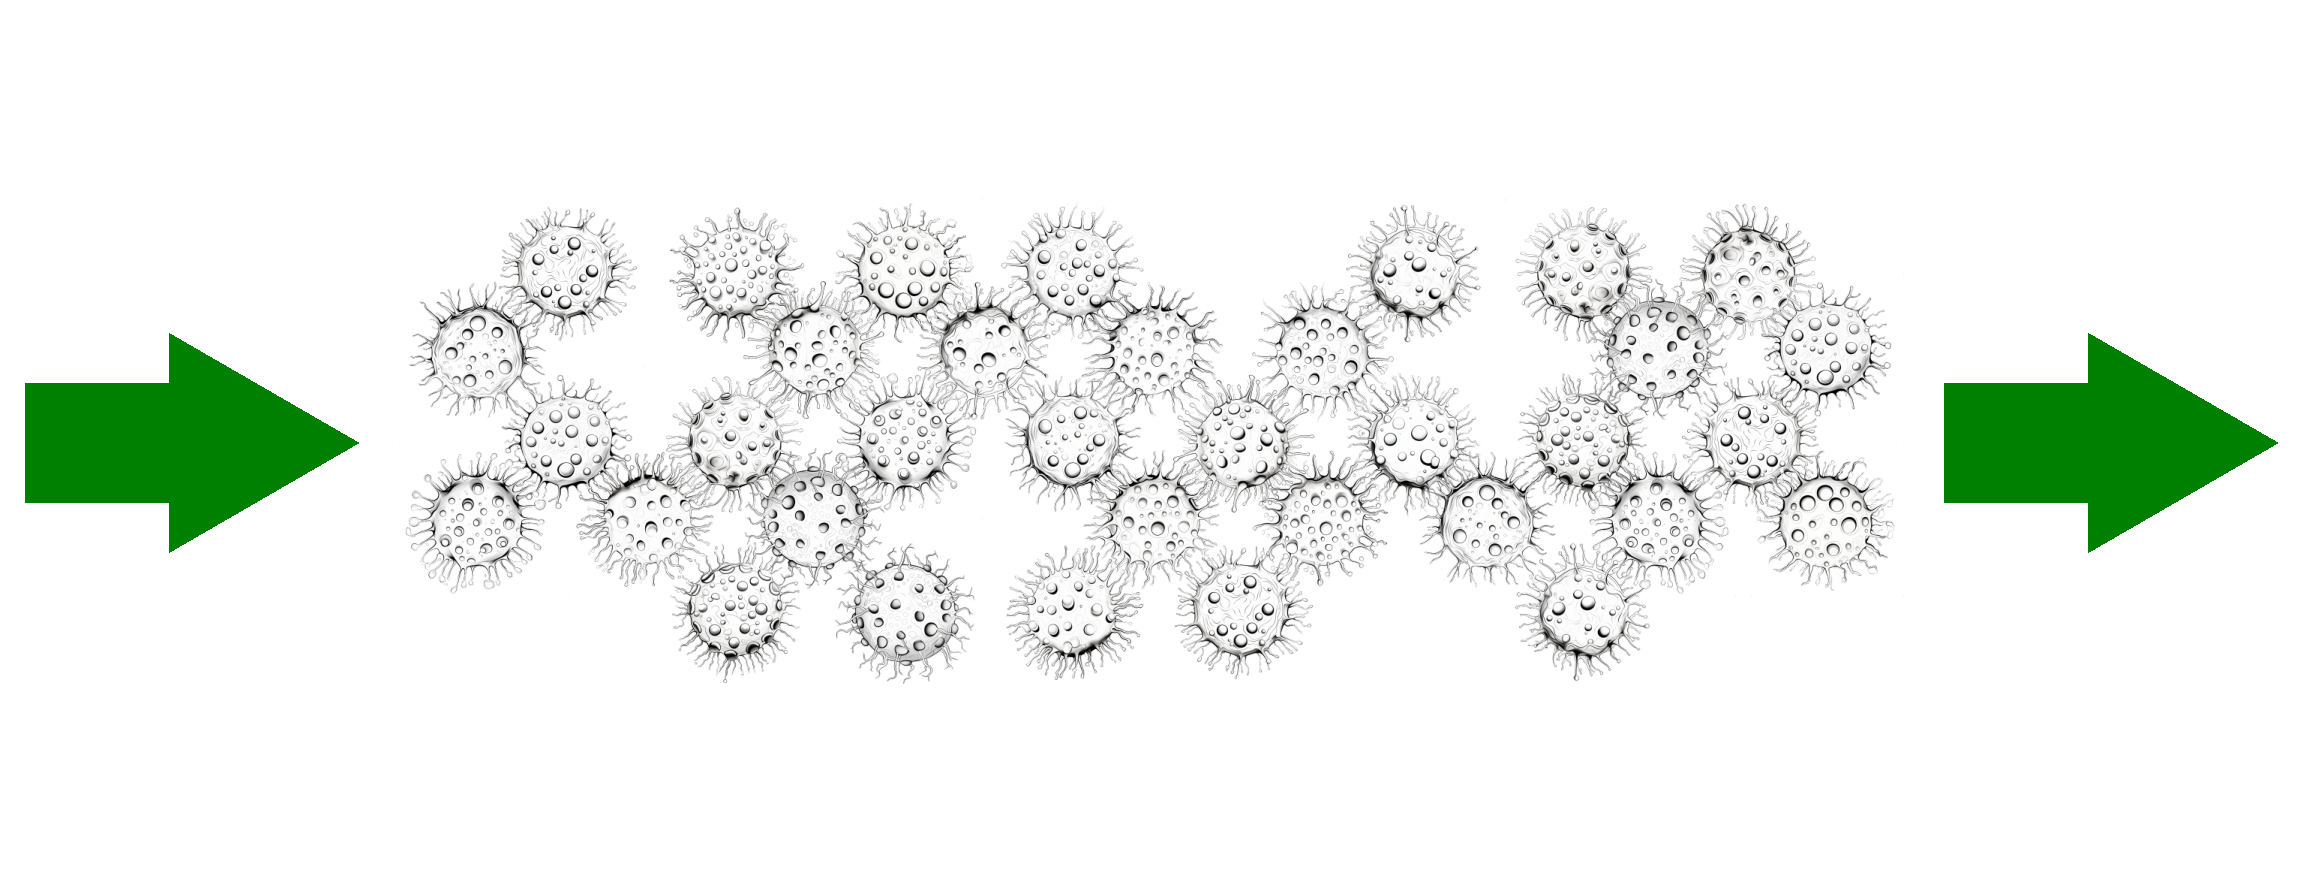
\includegraphics[width=\textwidth]{serial_heat_square_post.pdf}
			\vspace{0.5mm}
			\caption{Serial organ survives.}
		\end{subfigure}
		\vbar
		\begin{subfigure}[b]{0.35\textwidth}
			\addtocounter{subfigure}{-1}
			\renewcommand\thesubfigure{\alph{subfigure}2}
			\centering
			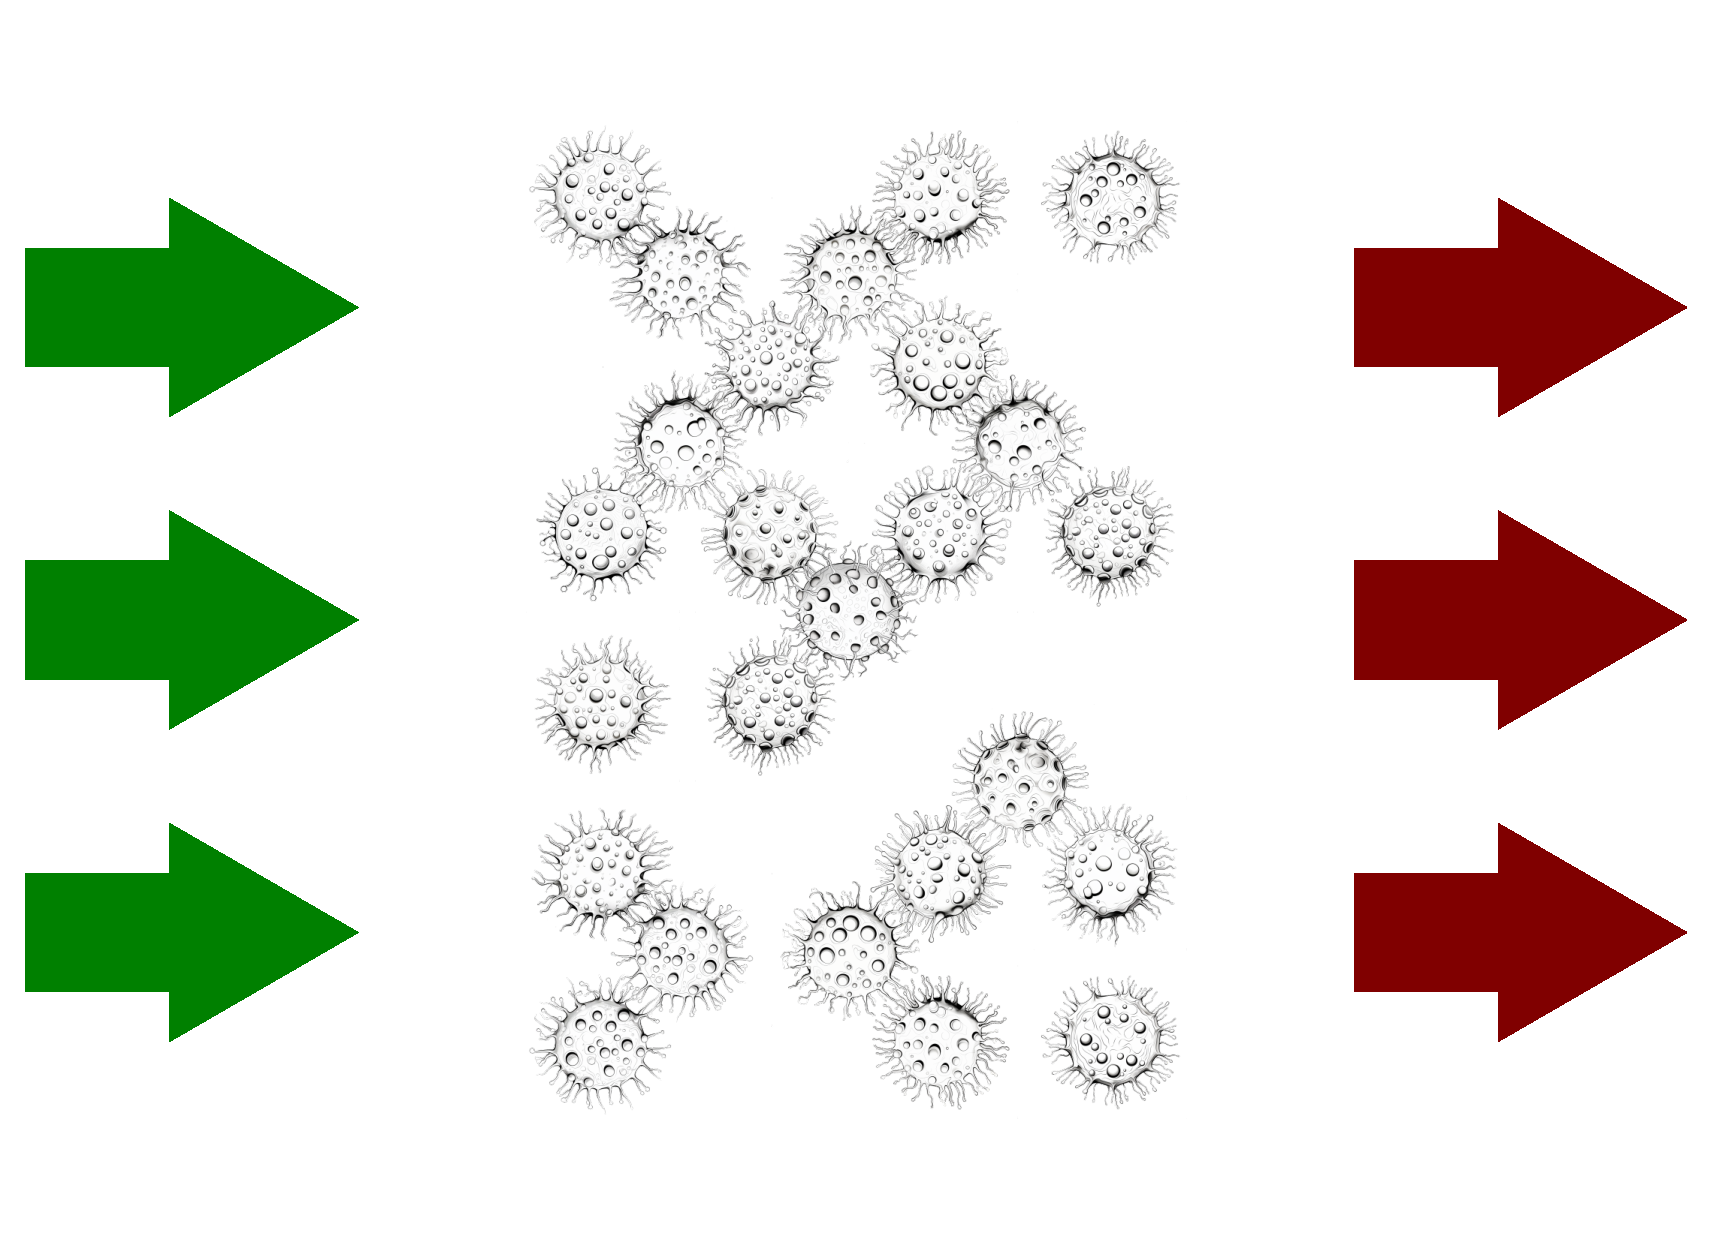
\includegraphics[width=\textwidth]{parallel_heat_square_post.pdf}
			\caption{Parallel organ dies.}
		\end{subfigure}	
	\end{subfigure}
	\addtocounter{subfigure}{-1}
	\caption{Irradiation type survival of organs serial-like and parallel-like.}
	\label{fig:serial_parallel_organ_radiation}	
\end{figure}

\subsection{Optimization Problem}

\paragraph{Ideal}
% minimize dose while reaching constraints

\paragraph{Practical}
% get as close as possible to meeting constraints
% building of cost function

\section{Dose Mimicking}
% principle
% => is a simpler problem
% => only works if dose to mimick is nearly acheaivable
% => can arise if machine is changing during treatment
% optim problem

\section{Optimization Algorithm Review for Dosimetry}
\subsection{Introduction}
% ArXiV paper

\subsection{Methods}
%Efficiently solving this optimization problem often involves designing the objective function to be convex, thereby providing a well-defined target for the optimization process.
%Gradient-based methods, Newtonian algorithms, or quasi-Newtonian algorithms are commonly employed for this purpose.
%We aim at benchmarking state-of-the-art open-source optimization algorithms for the specific task of radiotherapy dosimetry.

\subsection{Data}
% TG-119 \cite{AAPM-TG119}
\subsection{Objective function}
% details on the one used for this study
% => tested variations (p=1,2), changed importance factors, but v similar results
\subsection{Open-source Optimizers}
\paragraph{(Stochastic) Gradient Descent}
\paragraph{Conjugate Gradient}
\paragraph{Newton}
\paragraph{SLSQP}
\paragraph{RMSprop}
\paragraph{BFGS-based}
\subparagraph{Pure BFGS}
\subparagraph{L-BFGS}
\paragraph{Adam-based}
\subparagraph{Pure Adam}
\subparagraph{RAdam}
\subparagraph{NAdam}
\subparagraph{AdamDelta}
\subparagraph{Adamax}
\paragraph{Rprop}
\paragraph{Other optimizers variations}
%In addition, we also tested AdamW, Adagrad and ASGD.
%However, AdamW \& Adagrad behaved similarly to Adam, and ASGD behaved similarly to SGD.

\subsection{Results}
% 4 TGG-119 cases figures
\paragraph{Newton's method}
\paragraph{Best Algorithms}
\paragraph{LBFGS vs BFGS}

\subsection{Discussion}
